\documentclass{article}
\usepackage{graphicx}
\usepackage{float}
\usepackage[acronym]{glossaries}
\usepackage{fullpage}

\loadglsentries{acronyms}
\makeglossaries

\begin{document}

\begin{tabular}{rl}
  \textbf{Lab 7:} & DC Motor Configurations \\
  \textbf{Performed:} & March 11, 2013 \\
  \textbf{Partners:} & Rawley Dent \\ & Charles Pittman \\
  \textbf{Instructor:} & Dr. Weatherford
\end{tabular}

%\setlength\parindent{0pt}

\section*{Abstract}

In this experiment, the effect of a motor's construction on the torque-speed
relationship was examined.

\section*{Results}

\begin{figure}[H]
  \centering
    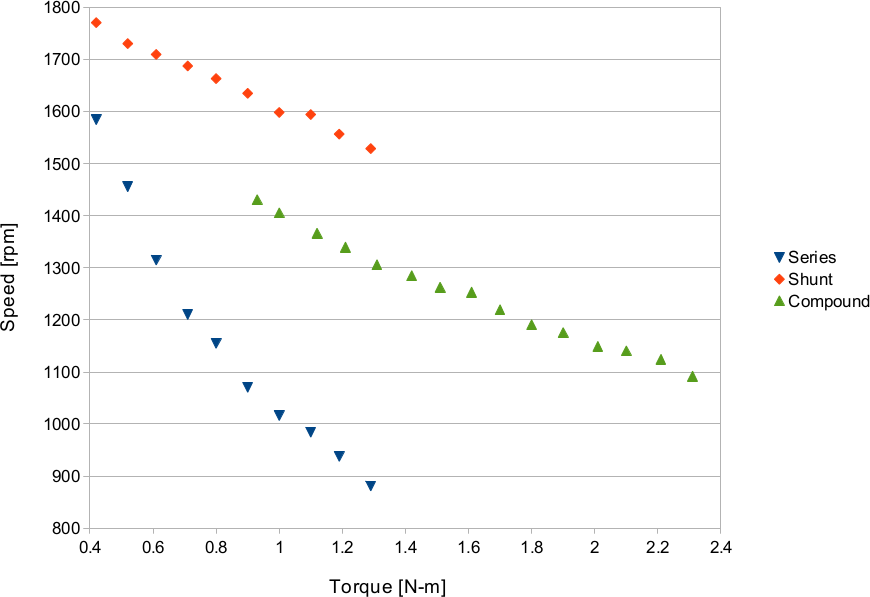
\includegraphics[width=0.6\textwidth]{img/graph}
    \caption{\textbf{Comparison of Speed vs. Torque Plots}}
    \label{fig:graph}
\end{figure}

\section*{Conclusions}

The torque-speed relationship, or terminal characteristics, of the shunt motor
resembles a straight line. In fact, the equation for a shunt motor’s speed vs\.
torque is a linear relationship with a negative slope. The terminal
characteristics of a series motor have a nonlinear relationship. It is noted
that as the torque on a series motor goes to zero, its speed goes to infinity.
However, the torque on a motor can never go to zero because of the mechanical,
core, and stray losses that must be overcome. Just as well, the speed of a
series motor can still turn fast enough to damage itself. The terminal
characteristics of a cumulatively compounded motor resemble both a series and a
shunt motor. This is because the compounded motor contains both a shunt and a
series field. Although the resemblance is hard to discern from Figure 1, if
more data was obtained, then at low torque, the compounded motor would most
resemble a shunt motor.  At higher torque the compounded motor would most
resemble a series motor.

%In Figure~\ref{fig:graph}, the linear relationship between DC motor speed
%$n_m$ and torque $\tau$ is exemplified.  The DC motor was initially operating
%at approximately 1500-rpm.  As the load torque was increased, the DC motor
%experienced a decrease in speed.  The armature current was also increasing
%while the load torque was increasing, and thus the internal generated voltage
%$E_A$ was decreased.

\end{document}
